% ============================================================================
%  "Present in Some Layer" Is Not Evidence
%  Build:  pdflatex main && bibtex main && pdflatex main && pdflatex main
%  Switches below control anonymity and the checklist. See README.md.
% ============================================================================
\documentclass{article}

% ---- switches ---------------------------------------------------------------
% \anontrue  = anonymized submission build (main.pdf)
% \anonfalse = non-anonymized build with a placeholder author block (main_named.pdf)
\newif\ifanon      \anontrue
\newif\ifchecklist \checklisttrue   % the NeurIPS checklist is mandatory; keep true

% Venue is not decided. Parameterized rather than guessed -- see paper/NOTES.md.
% NOTE: the official style emits "Submitted to <N>th Conference on NeurIPS (2026).
% Do not distribute." automatically in submission builds, and substitutes the track
% string only in the camera-ready (final) build. So the venue name is parameterized
% in the one place the style consumes it -- \workshoptitle -- rather than printed a
% second time by hand.
\newcommand{\venuename}{[WORKSHOP NAME]}

% Official NeurIPS 2026 style file (neurips_2026.sty, 2026-01-29), used verbatim.
% Track: workshop with double-blind reviewing. Change the track option here if the
% target venue changes; \workshoptitle sets the notice string.
\ifanon
  \usepackage[dblblindworkshop]{neurips_2026}
\else
  \usepackage[dblblindworkshop, final]{neurips_2026}
\fi
\workshoptitle{\venuename}

\usepackage{amsmath,amssymb}
\usepackage{booktabs}
\usepackage{graphicx}
\usepackage{xcolor}
\usepackage[hidelinks]{hyperref}
\usepackage{caption}
\usepackage{microtype}
\usepackage{enumitem}

\definecolor{bad}{HTML}{D55E00}
\definecolor{good}{HTML}{0072B2}
\newcommand{\code}[1]{\texttt{\small #1}}
\newcommand{\no}[1]{\textcolor{bad}{\textbf{#1}}}
\newcommand{\yes}[1]{\textcolor{good}{\textbf{#1}}}
\newcommand{\prov}{\textsuperscript{$\dagger$}}

\title{``Present in Some Layer'' Is Not Evidence:\\
Controls for Layer-Existence Claims in Mechanistic Interpretability}

% The style renders "Anonymous Author(s) / Affiliation / Address / email" itself
% when anonymous. No real name appears in this source in either build.
\ifanon\else
  % NB: a line here must not BEGIN with "[", or the style's tabular reads it as
  % the optional length argument of \\ and the build dies.
  \author{%
    \textbf{AUTHOR LIST TO BE CONFIRMED}\thanks{Placeholder. No real names are
    committed to this source file; fill in at camera-ready.}\\
    Affiliation to be confirmed\\
    \texttt{email@example.invalid}%
  }
\fi

\begin{document}
\maketitle

\begin{abstract}
A recurring inference in interpretability research reads: the correct answer
outranks a competitor at some intermediate layer, therefore the model
``represents the answer internally'' and fails only at readout. We show that this
inference is not merely weak but \emph{untestable as stated}. The statistic
behind it is an existence test taken as a maximum over $\sim$30 noisy
comparisons; two exchangeable series cross almost surely, and under the natural
label-swap null the statistic is \emph{invariant}, so its null distribution is a
point mass and no test exists. We demonstrate this first in simulation, with no
model and no data, and then as a case study on our own prior result. That result
reported that in 137 of 137 stale-state tracking failures in
Qwen2.5-7B-Instruct, the correct state outranks the stale state in at least one
internal depth, and concluded the update was encoded but unused. It fails four
controls. The reverse statistic holds in 137/137; the same test fires in 488/488
successes; the permutation null is degenerate; and the graded form of the
statistic is significant \emph{in the opposite direction} --- the correct state
wins fewer depths than label-swap chance. We further show that two figures we
had reported for the same quantity, a mean best rank of $47{,}343$ and of $2.3$,
are the same lens on the same 137 examples and differ only in which depths were
swept. Separately, the failure and success populations are completely confounded
on task condition. After matching and correcting for depth selection, two
signals survive: an attention-mass differential at depth 22 (matched
AUC $0.973$, held-out $0.970$) and, provisionally, a J-lens margin at depth 5
(matched $0.888$, held-out $0.882$). Logit-lens margin does not survive. Every
surviving result is correlational; none establishes that the measured quantity
participates in producing the output.
\end{abstract}

% =============================================================================
\section{Introduction}
% =============================================================================

Since the logit lens \citep{nostalgebraist2020logitlens}, a standard move in
interpretability has been to decode a model's intermediate residual stream into
vocabulary space and ask what the model ``already knows'' partway through its
computation. When the correct answer ranks above a competitor at some
intermediate depth but loses at the output, it is natural to conclude that the
information was present internally and that something went wrong at readout.
Claims of this shape appear across the literature, including in work arguing
that language models encode the correct answer while emitting an incorrect one
\citep{orgad2024llmsknow}.

The inference has a structural problem that is independent of the model, the
lens, and the task. Written out, the statistic is
\[
E \;=\; \mathbb{1}\!\left[\;\exists\,\ell \in \{0,\dots,L-1\} \;:\; r_\ell(c) < r_\ell(s)\;\right],
\]
an existence test over $L$ depths, i.e.\ a maximum over $L$ noisy comparisons.
Three consequences follow. First, $E$ saturates: two exchangeable rank series
cross at least once with probability approaching 1 well before $L = 30$, so
$E = 1$ carries almost no information. Second, and more seriously, $E$ has no
usable null. Under the natural null --- that the labels $c$ and $s$ are
exchangeable --- if both $E(c \succ s)$ and $E(s \succ c)$ hold in every example,
then swapping the labels cannot change the statistic's value. Its null
distribution is a point mass at the observed value, and there is nothing to test
against. Third, $E$ is blind to magnitude: it is satisfied identically whether
the correct answer reaches rank 2 or rank 40{,}000, and whether the competitor
is at rank 1 or rank 150{,}000.

This paper makes that argument concretely and then applies it. The case study is
our own earlier analysis. We had reported that in 137 of 137 stale-state
tracking failures, the correct state outranks the stale state in at least one
internal depth, and had drawn the encoded-but-unused conclusion. We now report
that this does not survive controls, and we retract it. We treat this as the
natural test case precisely because we know exactly how the number was produced
and can re-derive every figure from committed scripts.

\paragraph{Contributions.}
\begin{enumerate}[leftmargin=*,itemsep=1pt,topsep=2pt]
\item We characterize the existence-over-depth statistic and show, in simulation
      with no model or data, that it saturates, that its label-swap null is
      degenerate, and that it is insensitive to effect size and sign
      (Section~\ref{sec:nulls}).
\item We specify the two distinct permutation nulls such claims require --- a
      whole-example label swap, and an outcome shuffle with the maximum over
      depths taken \emph{inside} each permutation, which is a max-$T$ procedure
      \citep{westfall1993resampling,nichols2002permutation} --- and the depth
      bands that must be excluded to avoid circularity
      \citep{kriegeskorte2009circular}.
\item We apply these to a real claim of our own and report that it fails all
      four controls, including a graded form significant in the direction
      opposite the claim (Sections~\ref{sec:case}--\ref{sec:results}).
\item We show how two of our own reported figures for the same quantity differ
      by four orders of magnitude purely through depth-set selection, and give
      the matched, selection-corrected re-analysis that isolates what actually
      survives.
\end{enumerate}

% =============================================================================
\section{Background and related work}
% =============================================================================

\paragraph{Reading the residual stream.} The logit lens
\citep{nostalgebraist2020logitlens} applies the model's final norm and
unembedding to an intermediate residual state, effectively asking what the model
would predict if the remaining layers were the identity. The tuned lens
\citep{belrose2023tunedlens} fits an affine probe per layer to correct the
resulting bias. \citet{yomdin2024jump} learn linear ``shortcut'' transformations
that map a hidden state to a later-layer representation, bypassing the
intervening computation; this is the closest published relative of the J-lens
used in our case study, which linearizes the model's own remaining computation
rather than fitting a probe. \citet{geva2022ffn} analyze feed-forward updates
directly in vocabulary space. All of these make intermediate states readable,
and all of them invite the existence-style inference we examine.

\paragraph{Probing and its controls.} The methodological hazard is familiar from
the probing literature. \citet{hewitt2019control} introduced control tasks to
separate what a probe extracts from what it memorizes;
\citet{ravichander2021probing} showed that a property can be decodable from
representations without being used by the model for its task;
\citet{belinkov2022probing} surveys the shortcomings. Our point is the analogue
one level up: decodability at \emph{some} depth, selected post hoc, needs a null
and a control group in the same way probe accuracy does.

\paragraph{Selection and circularity.} Taking a maximum over depths and then
reporting the winner is a multiple-comparisons problem. The appropriate
correction is a max-$T$ permutation procedure, in which the maximum is
recomputed inside each permutation
\citep{westfall1993resampling,nichols2002permutation}. Selecting a depth on the
same data used to evaluate it is circular analysis
\citep{kriegeskorte2009circular}, and the space of defensible-looking analysis
choices --- which lens, which depths, which comparison group --- is a garden of
forking paths \citep{gelman2014forking}.

\paragraph{From correlation to cause.} Nothing in this paper is causal.
Establishing that a representation participates in producing an output requires
intervention: activation patching and its relatives
\citep{meng2022rome,wang2022ioi}, with the metric and corruption choices that
\citet{zhang2024patching} show materially change the conclusions. We specify
such an experiment in Appendix~\ref{app:patch} but did not have the compute to
run it.

% =============================================================================
\section{The statistic and its nulls}
\label{sec:nulls}
% =============================================================================

\paragraph{Notation.} Fix an example with a correct state $c$ and a competitor
state $s$. Let $\ell \in \{0,\dots,L-1\}$ index positions at which the residual
stream is read, and let $r_\ell(\cdot)$ be the rank of a token in the decoded
vocabulary distribution at position $\ell$, with rank 1 the argmax and smaller
meaning better. Define
\[
E \;=\; \mathbb{1}\big[\exists \ell : r_\ell(c) < r_\ell(s)\big],
\qquad
G \;=\; \textstyle\sum_{\ell} \mathbb{1}\big[r_\ell(c) < r_\ell(s)\big].
\]
$E$ is the existence statistic behind the claim type; $G$ is its graded form.

\paragraph{$E$ saturates and cannot be tested.}
Figure~\ref{fig:sim} makes both points without a model.
Panel~(a): for two exchangeable series, $P(E=1)$ rises steeply in $L$ and is
already $0.97$--$1.00$ at $L=29$ depending on noise; a series in which $c$ is
genuinely \emph{worse} than $s$ still yields $E=1$ about $92\%$ of the time.
Panel~(b): under Null A below, with $c$ given a genuine disadvantage, the null
distribution of $E$ has standard deviation $5\times10^{-4}$ and the observed
value sits inside it, whereas $G$ separates from its null by roughly 19 standard
deviations. Panel~(c): $E$ stays above $0.88$ across the entire range of true
effects, including where $c$ is worse, while $G$ moves monotonically. In the case
study $E=1$ in \emph{both} directions in every example, so the null is an exact
point mass and $p=1$ by construction.

\begin{figure}[t]
\centering
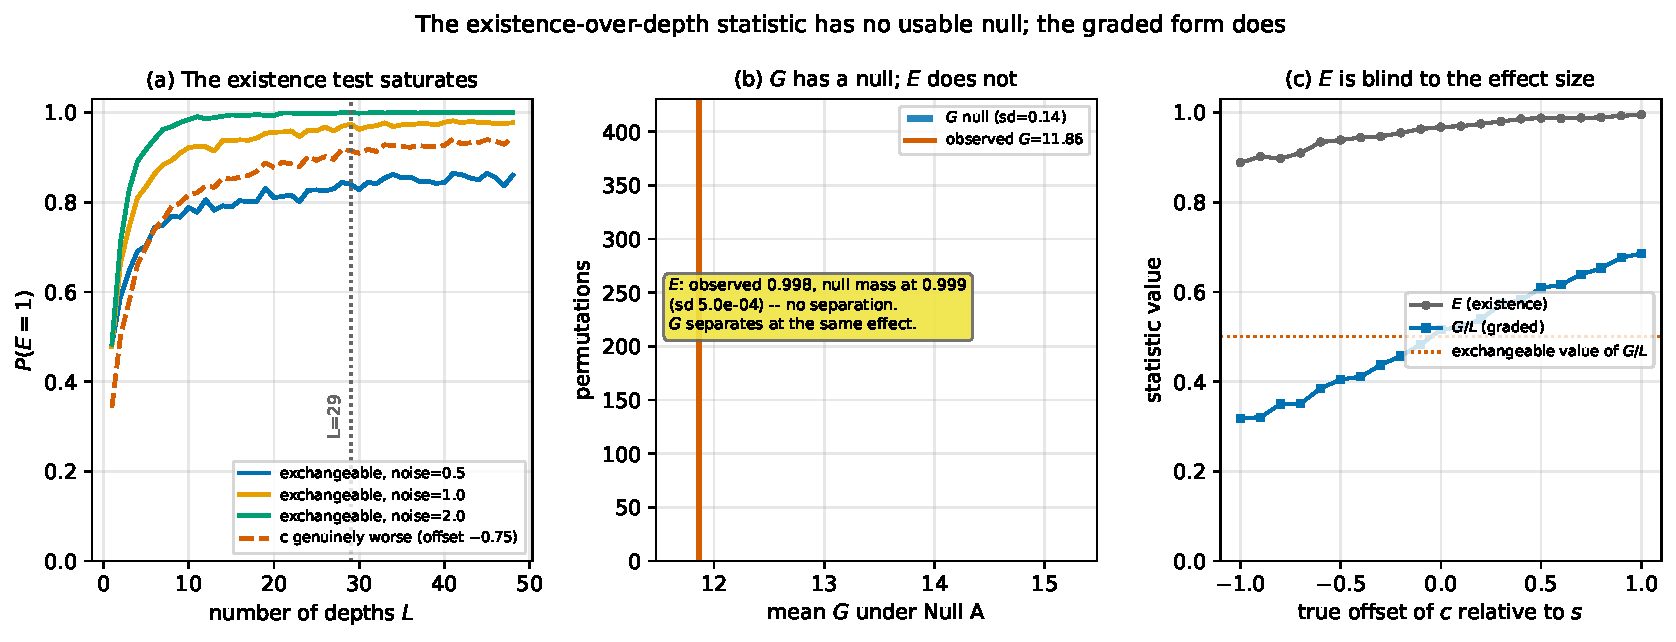
\includegraphics[width=\textwidth]{../../reports/existence_null_sim.pdf}
\caption{Model-free simulation (\code{sim/existence\_null\_sim.py}; seeded,
2{,}000 examples, 5{,}000 permutations). (a) The existence test saturates in the
number of depths, including when the correct state is genuinely worse. (b) With
a real effect present, $G$ separates from its null and $E$ does not. (c) $E$ is
insensitive to the size and sign of the effect.}
\label{fig:sim}
\end{figure}

\paragraph{Null A: whole-example label swap.} To test whether the identity of
the correct state carries information, swap $c$ and $s$ for an entire example
across all $L$ depths at once, and recompute the statistic. The swap must be
applied to the whole series. Swapping independently at each depth destroys
within-example cross-depth correlation and yields a falsely narrow null for a
maximum statistic --- it would make almost any $E$ look extreme.

\paragraph{Null B: outcome shuffle with the maximum inside.} To test whether a
per-depth measure separates two outcome groups, shuffle the group labels across
examples and, \emph{within each permutation}, recompute the measure at every
depth in the analysis band and take the maximum. Comparing the observed maximum
against this distribution is a max-$T$ procedure
\citep{westfall1993resampling,nichols2002permutation} and is what prices in
having chosen the best depth. Comparing a post-hoc-selected depth against a
per-depth null instead is the error this control exists to prevent.

\paragraph{Split-half depth selection.} Passing Null B shows that \emph{some}
depth separates the groups; it does not show that a \emph{particular} depth does.
We select the best depth on one half of the data and evaluate it on the held-out
half, repeatedly, and report both the held-out effect and how often each depth is
selected. A measure whose selected depth is not reproducible across splits does
not support a claim naming that depth.

\paragraph{Excluded bands.} Two ranges must be excluded before any
``internal'' claim. Positions adjacent to the embedding carry little of the
model's computation. Positions adjacent to the output are worse: at the final
residual position the lens is one norm and one unembedding away from the logits,
so it \emph{is} the model's decision, and any statistic separating outcomes
there is circular \citep{kriegeskorte2009circular}. In the case study a group
separation measured at the last position is exactly $1.000$ by construction.

% =============================================================================
\section{Case study: stale-state tracking}
\label{sec:case}
% =============================================================================

\paragraph{Task and data.} Each record narrates a sequence of entity movements
and then asks where one entity currently is. Exactly one relocation makes an
earlier stated location stale; a failure is the model emitting the stale room.
The dataset is 5{,}000 synthetic records varying complexity level, entity type
(agent or object), and the number and position of distractor mentions.

\paragraph{Model and configuration.} Qwen2.5-7B-Instruct in bfloat16, eager
attention (required to capture attention probabilities), no quantization, chat
prompt format, with an entity-aware prefill ending exactly where the room name
must appear; the readout is the single token at that position. All three runs
used \code{transformers} 5.14.1. Per-run configurations are committed.

\paragraph{Depth indexing.} The model has 28 decoder layers. A pre-hook on the
input of each layer plus a post-hook on the output of the last gives
\textbf{29 residual-stream positions}, depths $0..28$; depth 28 is the final
residual stream, immediately before the final norm and unembedding. Attention is
indexed by decoder layer, $0..27$, so \textbf{no attention exists at depth 28} ---
a structural fact, not a capture failure. We say ``depths'' rather than
``layers'' throughout. Ranks are 1-based and the vocabulary is $V = 152{,}064$.

\paragraph{Runs.} Three runs, all from the same 5{,}000-record dataset
(Table~\ref{tab:runs}). Behaviourally the model answers correctly on $97.1\%$ of
records, emits the stale state on $2.7\%$ ($137$ records), and produces an
unparseable answer on $0.2\%$. The 137-failure run is the complete failure
population, re-swept at all depths. Reconstructing this required signature
matching, because that export renumbered example identifiers
(Appendix~\ref{app:provenance}); the twelve failures common to both full-depth
runs agree exactly on every rank column, so the two pool.

\begin{table}[t]
\centering\small
\begin{tabular}{lrrl}
\toprule
Run & Records & Depths & Outcomes \\
\midrule
5k, three depths      & 5{,}000 & 3 ($5,8,13$) & 4{,}853 correct / 137 stale / 10 other \\
500, full sweep       & 500     & 29 ($0..28$) & 488 correct / 12 stale \\
137 failures, full sweep & 137  & 29 ($0..28$) & 137 stale \\
\bottomrule
\end{tabular}
\caption{The three runs. The 500-record run is a subset of the 5k dataset; the
137-failure run is its complete failure population.}
\label{tab:runs}
\end{table}

\paragraph{Measures.} \emph{Logit lens}: $\mathrm{unembed}(\mathrm{norm}(h_\ell))$.
\emph{J-lens}: a first-order expansion of the model's own remaining computation,
$f_\ell(0) + J h_\ell$, where $f_\ell$ runs decoder layers $\ell..28$ with the
real frozen KV cache. Nine attention columns record mass at the readout position.
For each measure we use the margin between $c$ and $s$.

% =============================================================================
\section{Results}
\label{sec:results}
% =============================================================================

\subsection{The claim fails four controls}

\begin{table}[t]
\centering\small
\begin{tabular}{llr}
\toprule
Control & What it asks & Result \\
\midrule
Symmetry & Does $E$ also hold with $c$ and $s$ swapped? & \no{137/137 $=100\%$} \\
Discrimination & Does $E$ also hold on successes?      & \no{488/488 $=100\%$} \\
Null A, $E$    & Is $E$ testable under label swap?      & \no{point mass, $p=1.00$} \\
Null A, $G$    & Is the graded form as claimed?         & \no{$10.93$ vs null $14.48$, $p<10^{-4}$} \\
\bottomrule
\end{tabular}
\caption{The four controls on the original claim (logit lens; J-lens is
identical on the first three and gives $G=8.41$ vs null $14.34$, $p<10^{-4}$).
Every entry falsifies the claim.}
\label{tab:controls}
\end{table}

Table~\ref{tab:controls} summarizes. The existence test fires in both directions
in every failure, and in every success. Under Null A it is invariant: because
both directions already hold in all 137 examples, relabelling cannot move it, so
the null is an exact point mass and $p=1.00$. This is the difference between a
statistic that is non-significant and one that is untestable; $E$ is the latter.

The graded statistic $G$ \emph{is} testable, and it points the other way. The
correct state wins $10.93$ of 29 depths on average, against a label-swap null of
$14.48$ (95\% interval $[13.12, 15.82]$), $p<10^{-4}$. Under J-lens, $8.41$
against $14.34$. \textbf{The correct state wins fewer depths than chance under
label exchange} --- a finding in its own right, and the opposite of what the
original claim asserted.

\subsection{Two reported figures for one quantity}

We had separately reported a mean best rank for the correct state of $47{,}343$
and of $2.3$. These are the same lens on the same 137 examples. The only
difference is the depth set over which the minimum is taken: $\{5,8,13\}$ gives
$47{,}343.5$; all 29 depths give $2.3$. Restricting the full sweep to
$\{5,8,13\}$ reproduces $47{,}343.5$ exactly.

The favourable figure is an artifact of admitting output-committed depths, and
inspecting where the minimum falls shows why it cannot support the claim. The
best rank occurs at depth $\geq 26$ in \emph{100\%} of failures, and at that
depth the correct state outranks the stale state in only $13.1\%$ of cases: the
median stale rank there is $1$ and the median correct rank is $2$. The correct
state is the runner-up at the output, which is what a stale failure \emph{is}.
Where the correct state genuinely wins by the largest margin (median depth 9),
both tokens are buried --- median ranks $24{,}183$ against $103{,}440$ out of
$152{,}064$. The two regimes are disjoint, and the original claim was assembled
by taking the existence test from one and the impressive rank from the other.

\subsection{The comparison groups are confounded}

Every failure is a complexity-3, agent-entity, middle-distractor record; $70.7\%$
of successes contain no distractors at all, and only $29.3\%$ are complexity-3.
Any measure tracking task difficulty separates these groups for reasons unrelated
to the outcome. We therefore define a matched stratum (complexity 3, agent,
middle distractor, 3--4 distractors), which retains $72$ of $488$ successes at
full depth and $682$ of $4{,}853$ in the three-depth run; all 137 failures
already lie inside it. Figure~\ref{fig:rawmatched} shows the cost of ignoring
this: at depth 13 the J-lens AUC falls from $0.952$ to $0.700$ under matching.

Controls 1 and 3 above are within-failure analyses and are untouched by the
confound; control 2's conclusion also stands, since a statistic at $100\%$ in
both arms cannot be rescued by rebalancing. What the confound invalidates is
every \emph{magnitude} computed on unmatched groups.

\begin{figure}[t]
\centering
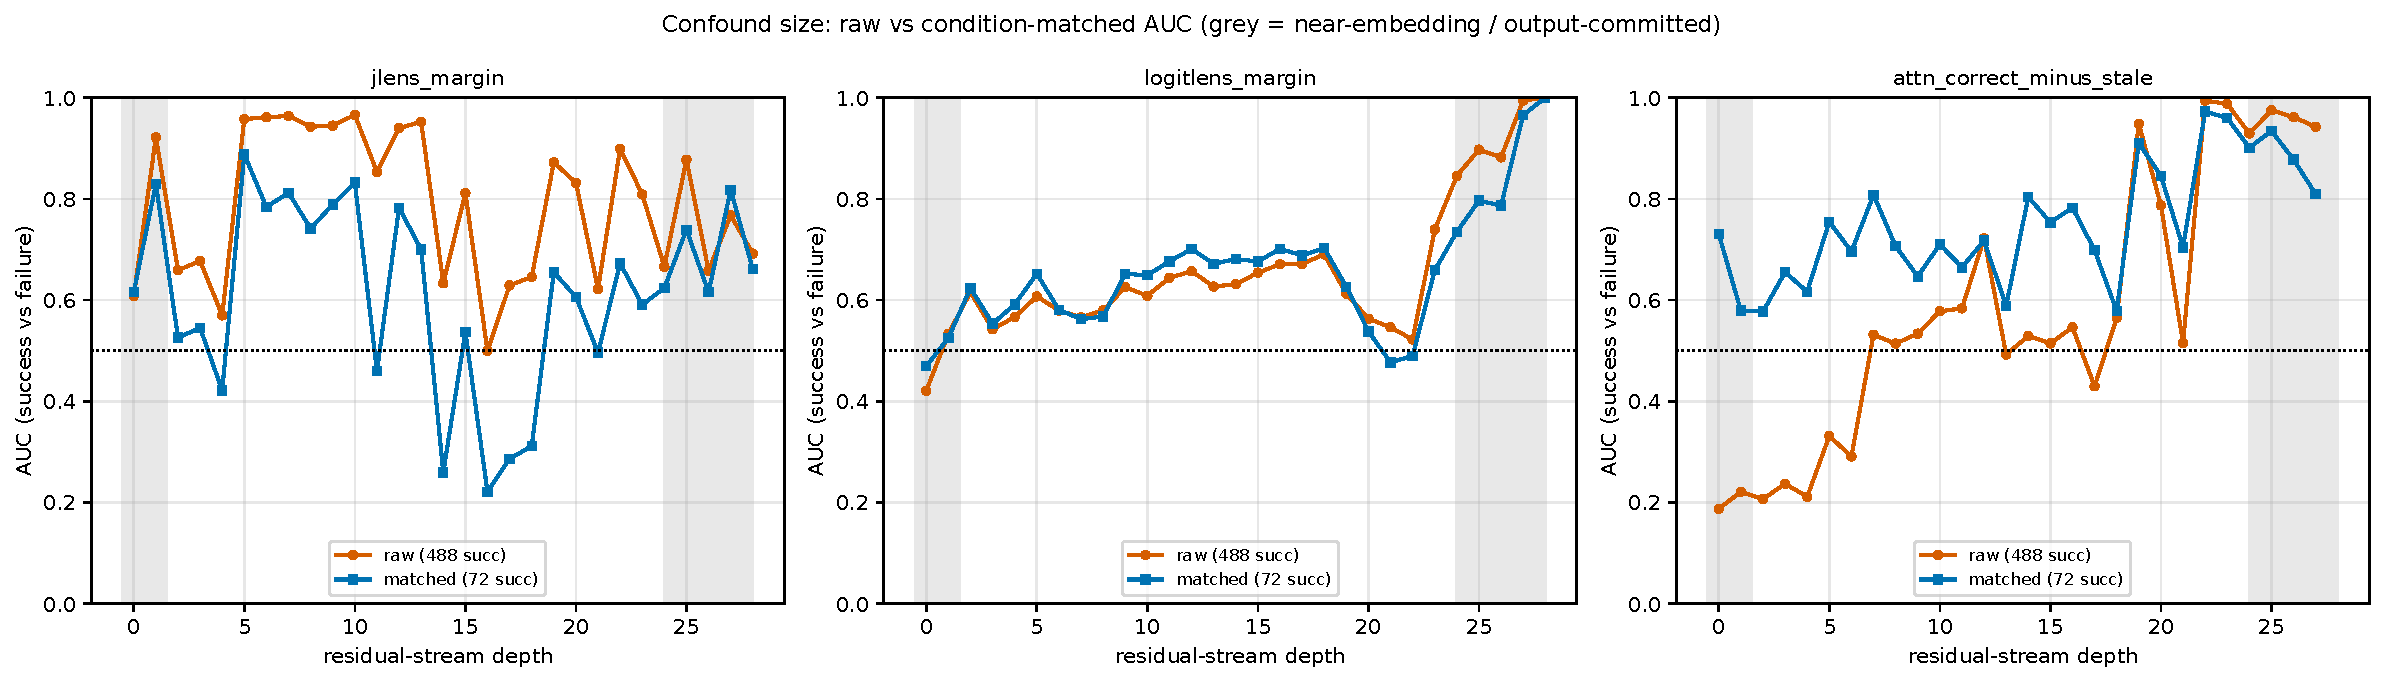
\includegraphics[width=\textwidth]{../../reports/auc_raw_vs_matched.pdf}
\caption{Per-depth AUC separating success from failure, raw (488 successes)
versus condition-matched (72). Shaded bands are the excluded near-embedding and
output-committed positions; at depth 28 the raw AUC is exactly $1.000$ because
the lens there is the model's decision.}
\label{fig:rawmatched}
\end{figure}

\subsection{What survives}

\begin{table}[t]
\centering\small
\begin{tabular}{lrrrrrl}
\toprule
Measure & Depth & Raw & Matched & Null B $p$ & Held-out & Depth stability \\
\midrule
\code{attn\_correct\_minus\_stale} & 22 & $0.994$ & $0.973$ & $<10^{-4}$ & $0.970$ & \yes{$90\%$} \\
\code{jlens\_margin}\prov          & 5  & $0.958$ & $0.888$ & $<10^{-4}$ & $0.882$ & \yes{$96\%$} \\
\code{logitlens\_margin}           & 18 & $0.690$ & $0.703$ & $<10^{-4}$ & $0.669$ & \no{$32\%$} \\
\bottomrule
\end{tabular}
\caption{Matched, selection-corrected results. Depth is the one split-half
actually selects; stability is the fraction of 500 splits selecting it.
\prov J-lens results are provisional pending replay validation
(Section~\ref{sec:limits}).}
\label{tab:survive}
\end{table}

Table~\ref{tab:survive} gives the matched, selection-corrected picture. Two
measures survive all three controls. Attention mass differential at depth 22
separates the groups with matched AUC $0.973$ and held-out $0.970$, selecting
depth 22 in $90\%$ of splits; failures place more mass on the stale anchor and
less on the update mention. J-lens margin at depth 5 gives matched $0.888$,
held-out $0.882$, depth 5 selected in $96\%$ of splits, replicating at $0.883$
against the larger matched control set in the three-depth run.

\textbf{Logit-lens margin does not survive.} It clears Null B, but the depth it
selects is reproducible in only $32\%$ of splits, spreading across depths 12, 16,
18 and 23. The effect is real but diffuse, and no claim naming a specific
logit-lens depth is supported. This is precisely the distinction the split-half
control exists to draw, and it is invisible to a permutation test alone.

The full attention sweep (Figure~\ref{fig:attn}) locates discrimination at depths
19--25 and near chance through the early and middle stack. Within the matched
stratum two column pairs are identical, because matched records carry a single
stale mention, so the sweep covers seven distinct measures rather than nine.

\begin{figure}[t]
\centering
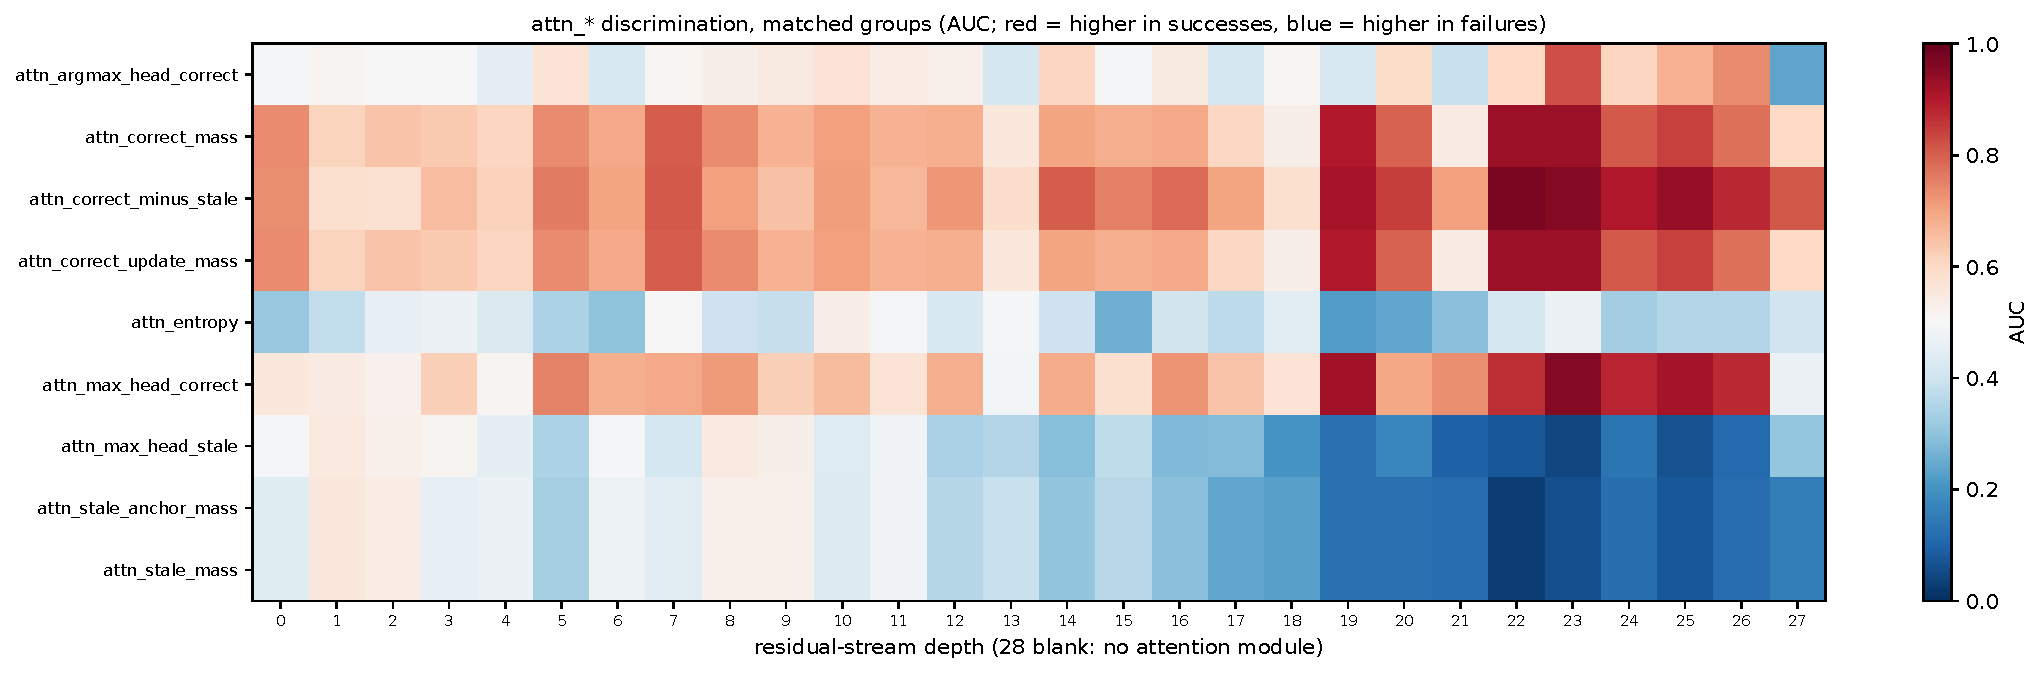
\includegraphics[width=\textwidth]{../../reports/attn_sweep_matched.pdf}
\caption{Matched attention sweep, all nine columns across depths $0..27$
(depth 28 has no attention module). AUC below $0.5$ means the quantity is higher
in failures.}
\label{fig:attn}
\end{figure}

% =============================================================================
\section{Limitations}
\label{sec:limits}
% =============================================================================

\paragraph{J-lens validity is unresolved; its results are provisional.}
The probe ships a self-check that replays the truncated stack from depth 0 and
compares against the real forward pass. \textbf{It was not enabled for any of the
three runs behind this paper} --- all three configurations record
\code{self\_check: false}. We therefore have no replay validation for the J-lens
numbers reported here, and we label them provisional. Auditing that code for this
paper also surfaced two defects, now fixed: the failure branch compared
\code{diff > 0.5}, and since \code{nan > 0.5} is false in IEEE 754, a run whose
logits went non-finite printed ``OK''; and the docstring named a tolerance of
$\sim$$10^{-1}$ while the code used $0.5$. We additionally note that
$\max|\Delta\text{logit}|$ over a $152{,}064$-token vocabulary can be dominated by
a deep-tail token carrying no probability mass, so the check now also reports KL
between the two softmaxes. A dtype-ladder diagnostic exists
(Appendix~\ref{app:jlens}) but has not been run. Until it is, the depth-5 J-lens
result should be read as provisional. The attention result does not depend on
J-lens.

\paragraph{What J-lens measures even if valid.} By construction
$f_\ell$ executes decoder layers $\ell..28$ with the real KV cache, so J-lens at
depth 5 includes the entire downstream network. We tested whether this makes it a
disguised readout of the output and found it is not. On the matched groups, the
depth-specific component alone --- after removing each example's cross-depth
mean --- still gives AUC $0.871$ at depth 5 against a matched $0.888$, and
cross-depth rank correlation is markedly \emph{lower} for J-lens ($0.268$) than
for the logit lens ($0.538$), which is the opposite of what a shared
output-driven component would produce. The licensed statement is nonetheless
``decodable \emph{through the remaining network}'', not ``represented at depth
5''. Under the logit lens, which does not route through downstream layers,
matched internal AUC is $0.57$--$0.62$ everywhere: no usable internal signal.

\paragraph{Statistical power.} The matched full-depth comparison rests on 72
successes. The three-depth run supplies 682 matched successes but only at depths
5, 8 and 13. The failure population is capped at 137 --- that is every failure
this configuration produces, so a larger failure sample requires a harder task,
not more sampling.

\paragraph{Everything here is correlational.} A measure that predicts an outcome
need not participate in producing it. We specify a patching experiment with its
controls in Appendix~\ref{app:patch}, including a control for the failure mode in
which a patch at the decision token simply transfers a donor's answer --- which
is answer-copying, not localization --- but we did not have the compute to run
it. No claim in this paper is causal.

\paragraph{Scope.} One model, one synthetic dataset, one prompt template. The
concentration of all failures in a single condition cell limits external validity
independently of the statistical issues.

% =============================================================================
\section{Recommendations}
\label{sec:reco}
% =============================================================================

\begin{enumerate}[leftmargin=*,itemsep=2pt,topsep=2pt]
\item \textbf{Do not report an existence-over-depth statistic as evidence.} If
      both directions hold in every example it is untestable, not merely weak.
      Report the graded form, which has a null.
\item \textbf{State the depth set with every depth-selected statistic.} Two of
      our own figures for one quantity differed by four orders of magnitude
      through depth-set choice alone, and the discrepancy is unrecoverable from
      the numbers.
\item \textbf{Exclude output-committed positions from ``internal'' claims.} At
      the last residual position the lens is the decision, and the statistic is
      circular \citep{kriegeskorte2009circular}.
\item \textbf{Match the comparison groups, and report raw beside matched} so the
      confound size stays visible.
\item \textbf{Correct for depth selection twice}: a max-$T$ permutation for
      whether any depth separates the groups, and split-half selection for
      whether a named depth reproducibly does. The second caught a result the
      first passed.
\end{enumerate}

The effect of these is to raise the evidentiary bar for a common class of
interpretability claim, including one of our own. We think the trade is
favourable: of the results we previously reported, the two that survive are
better localized and better supported than the one we lost.

\bibliographystyle{plainnat}
\bibliography{refs}

\appendix
\newpage
\section{Provenance reconstruction}
\label{app:provenance}
The 137-failure export renumbered \code{example\_id} and \code{dataset\_index}
to $0..136$, so it appears disjoint from the parent run under an index join. We
recovered the mapping by matching per-example rank signatures at the three
depths the runs share; all 137 signatures are unique and all 137 match. The
twelve failures present in both full-depth runs agree exactly on every rank
column, which is what licenses pooling them into a single
137-versus-488 comparison. An earlier version of this analysis used only the
twelve failures inside the 500-record run, an avoidable loss of power.

\section{Planned patching experiment}
\label{app:patch}
For each of the 137 failures, patch attention-head outputs at depths 19--22 from
a condition-matched success in the same cell, and measure the rate at which the
output flips to the correct room. Controls: random heads at the same depths;
heads ranked lowest by the committed head ranking; and mean-ablation of the
top-$k$ stale-preferring heads. A patch applied at the decision token can
transfer the donor's answer outright, which is answer-copying rather than
localization; the donor-mismatch control detects this. Metrics and corruption
choices follow \citet{zhang2024patching}. Script: \code{patch\_probe.py}.
\textbf{Not run: no GPU was available.}

\section{J-lens replay diagnostic}
\label{app:jlens}
\code{jlens\_diag.py} runs bf16 and fp16 arms plus a small-model dtype ladder and
computes KL between the replayed and real softmaxes. If fp32 gives KL on the
order of $10^{-4}$ while bf16 is order 1, the discrepancy is numerical precision
rather than a fault in the truncated stack. \textbf{Not run: no GPU was
available.}

\section{Reproduction}
\label{app:repro}
Every number in this paper is produced by a committed script over committed CSVs.
No GPU is required.
\begin{quote}\code{python3 controls\_check.py}\\
\code{python3 controls\_check2.py}\\
\code{python3 sim/existence\_null\_sim.py}\end{quote}
Outputs land in \code{reports/}. Seeds are fixed (5{,}000 permutations,
500 splits). The paper pulls its figures from \code{reports/} at build time.

\section{LLM usage}
\label{app:llm}
The analysis, controls and this manuscript were developed with the assistance of
a large language model acting as a coding and analysis assistant. All statistical
procedures were specified by the authors; all code and results are reproducible
from the committed scripts, and every number in the paper is traceable to a
script output file. No model or vendor names are given in this build.

\ifchecklist
\newpage
\section*{NeurIPS Paper Checklist}




\begin{enumerate}

\item {\bf Claims}
    \item[] Question: Do the main claims made in the abstract and introduction accurately reflect the paper's contributions and scope?
    \item[] Answer: \answerYes{} % Replace by \answerYes{}, \answerNo{}, or \answerNA{}.
    \item[] Justification: The abstract and introduction state that the critiqued claim was our own prior analysis, that it fails four controls, that one signal survives matching and selection correction, that a second measure passing the same tests is demoted to exploratory because the lens producing it fails a convergence check, and that every surviving result is correlational. No causal claim is made anywhere.
    \item[] Guidelines:
    \begin{itemize}
        \item The answer \answerNA{} means that the abstract and introduction do not include the claims made in the paper.
        \item The abstract and/or introduction should clearly state the claims made, including the contributions made in the paper and important assumptions and limitations. A \answerNo{} or \answerNA{} answer to this question will not be perceived well by the reviewers. 
        \item The claims made should match theoretical and experimental results, and reflect how much the results can be expected to generalize to other settings. 
        \item It is fine to include aspirational goals as motivation as long as it is clear that these goals are not attained by the paper. 
    \end{itemize}

\item {\bf Limitations}
    \item[] Question: Does the paper discuss the limitations of the work performed by the authors?
    \item[] Answer: \answerYes{} % Replace by \answerYes{}, \answerNo{}, or \answerNA{}.
    \item[] Justification: Section~\ref{sec:limits} (Limitations) covers why the J-lens result is exploratory --- the probe computes $f_\ell(0) + J_\ell(h_\ell)h_\ell$, which is not a first-order expansion and fails to converge to the model's output as $\ell \to 28$ --- together with the two self-check defects we found, the 72-success ceiling on the matched full-depth comparison, the 137-failure cap, single model and single synthetic dataset, and the total absence of causal evidence.
    \item[] Guidelines:
    \begin{itemize}
        \item The answer \answerNA{} means that the paper has no limitation while the answer \answerNo{} means that the paper has limitations, but those are not discussed in the paper. 
        \item The authors are encouraged to create a separate ``Limitations'' section in their paper.
        \item The paper should point out any strong assumptions and how robust the results are to violations of these assumptions (e.g., independence assumptions, noiseless settings, model well-specification, asymptotic approximations only holding locally). The authors should reflect on how these assumptions might be violated in practice and what the implications would be.
        \item The authors should reflect on the scope of the claims made, e.g., if the approach was only tested on a few datasets or with a few runs. In general, empirical results often depend on implicit assumptions, which should be articulated.
        \item The authors should reflect on the factors that influence the performance of the approach. For example, a facial recognition algorithm may perform poorly when image resolution is low or images are taken in low lighting. Or a speech-to-text system might not be used reliably to provide closed captions for online lectures because it fails to handle technical jargon.
        \item The authors should discuss the computational efficiency of the proposed algorithms and how they scale with dataset size.
        \item If applicable, the authors should discuss possible limitations of their approach to address problems of privacy and fairness.
        \item While the authors might fear that complete honesty about limitations might be used by reviewers as grounds for rejection, a worse outcome might be that reviewers discover limitations that aren't acknowledged in the paper. The authors should use their best judgment and recognize that individual actions in favor of transparency play an important role in developing norms that preserve the integrity of the community. Reviewers will be specifically instructed to not penalize honesty concerning limitations.
    \end{itemize}

\item {\bf Theory assumptions and proofs}
    \item[] Question: For each theoretical result, does the paper provide the full set of assumptions and a complete (and correct) proof?
    \item[] Answer: \answerNA{} % Replace by \answerYes{}, \answerNo{}, or \answerNA{}.
    \item[] Justification: The paper contains no theorems. Its one analytic observation---that the existence statistic is invariant under the whole-example label swap when both directions hold in every example, so its null is a point mass---is immediate from the definition and is stated inline in Section~\ref{sec:nulls}, then confirmed empirically by a 5{,}000-permutation test.
    \item[] Guidelines:
    \begin{itemize}
        \item The answer \answerNA{} means that the paper does not include theoretical results. 
        \item All the theorems, formulas, and proofs in the paper should be numbered and cross-referenced.
        \item All assumptions should be clearly stated or referenced in the statement of any theorems.
        \item The proofs can either appear in the main paper or the supplemental material, but if they appear in the supplemental material, the authors are encouraged to provide a short proof sketch to provide intuition. 
        \item Inversely, any informal proof provided in the core of the paper should be complemented by formal proofs provided in appendix or supplemental material.
        \item Theorems and Lemmas that the proof relies upon should be properly referenced. 
    \end{itemize}

    \item {\bf Experimental result reproducibility}
    \item[] Question: Does the paper fully disclose all the information needed to reproduce the main experimental results of the paper to the extent that it affects the main claims and/or conclusions of the paper (regardless of whether the code and data are provided or not)?
    \item[] Answer: \answerYes{} % Replace by \answerYes{}, \answerNo{}, or \answerNA{}.
    \item[] Justification: Every number is produced by a committed script over committed CSVs and copied from its output file; none is entered by hand. Seeds are fixed (5{,}000 permutations, 500 splits). The rebuild sequence is in Appendix~\ref{app:repro}. No GPU is needed to reproduce any result in the paper.
    \item[] Guidelines:
    \begin{itemize}
        \item The answer \answerNA{} means that the paper does not include experiments.
        \item If the paper includes experiments, a \answerNo{} answer to this question will not be perceived well by the reviewers: Making the paper reproducible is important, regardless of whether the code and data are provided or not.
        \item If the contribution is a dataset and\slash or model, the authors should describe the steps taken to make their results reproducible or verifiable. 
        \item Depending on the contribution, reproducibility can be accomplished in various ways. For example, if the contribution is a novel architecture, describing the architecture fully might suffice, or if the contribution is a specific model and empirical evaluation, it may be necessary to either make it possible for others to replicate the model with the same dataset, or provide access to the model. In general. releasing code and data is often one good way to accomplish this, but reproducibility can also be provided via detailed instructions for how to replicate the results, access to a hosted model (e.g., in the case of a large language model), releasing of a model checkpoint, or other means that are appropriate to the research performed.
        \item While NeurIPS does not require releasing code, the conference does require all submissions to provide some reasonable avenue for reproducibility, which may depend on the nature of the contribution. For example
        \begin{enumerate}
            \item If the contribution is primarily a new algorithm, the paper should make it clear how to reproduce that algorithm.
            \item If the contribution is primarily a new model architecture, the paper should describe the architecture clearly and fully.
            \item If the contribution is a new model (e.g., a large language model), then there should either be a way to access this model for reproducing the results or a way to reproduce the model (e.g., with an open-source dataset or instructions for how to construct the dataset).
            \item We recognize that reproducibility may be tricky in some cases, in which case authors are welcome to describe the particular way they provide for reproducibility. In the case of closed-source models, it may be that access to the model is limited in some way (e.g., to registered users), but it should be possible for other researchers to have some path to reproducing or verifying the results.
        \end{enumerate}
    \end{itemize}


\item {\bf Open access to data and code}
    \item[] Question: Does the paper provide open access to the data and code, with sufficient instructions to faithfully reproduce the main experimental results, as described in supplemental material?
    \item[] Answer: \answerYes{} % Replace by \answerYes{}, \answerNo{}, or \answerNA{}.
    \item[] Justification: The repository is private at submission time and will be made public at camera-ready; its URL is withheld here and will be added then. An archive accompanies the submission (\texttt{supplementary\_anon.zip}), anonymized regardless of build, containing the analysis scripts, the simulation, the committed per-depth CSVs and per-run configuration files, every generated output in \texttt{reports/}, and a README with the rebuild commands. It carries no git history, names or URLs.
    \item[] Guidelines:
    \begin{itemize}
        \item The answer \answerNA{} means that paper does not include experiments requiring code.
        \item Please see the NeurIPS code and data submission guidelines (\url{https://neurips.cc/public/guides/CodeSubmissionPolicy}) for more details.
        \item While we encourage the release of code and data, we understand that this might not be possible, so \answerNo{} is an acceptable answer. Papers cannot be rejected simply for not including code, unless this is central to the contribution (e.g., for a new open-source benchmark).
        \item The instructions should contain the exact command and environment needed to run to reproduce the results. See the NeurIPS code and data submission guidelines (\url{https://neurips.cc/public/guides/CodeSubmissionPolicy}) for more details.
        \item The authors should provide instructions on data access and preparation, including how to access the raw data, preprocessed data, intermediate data, and generated data, etc.
        \item The authors should provide scripts to reproduce all experimental results for the new proposed method and baselines. If only a subset of experiments are reproducible, they should state which ones are omitted from the script and why.
        \item At submission time, to preserve anonymity, the authors should release anonymized versions (if applicable).
        \item Providing as much information as possible in supplemental material (appended to the paper) is recommended, but including URLs to data and code is permitted.
    \end{itemize}


\item {\bf Experimental setting/details}
    \item[] Question: Does the paper specify all the training and test details (e.g., data splits, hyperparameters, how they were chosen, type of optimizer) necessary to understand the results?
    \item[] Answer: \answerYes{} % Replace by \answerYes{}, \answerNo{}, or \answerNA{}.
    \item[] Justification: Section~\ref{sec:case} gives the model, precision, attention implementation, prompt format, prefill and readout position, and the composition of all three runs; Appendix~\ref{app:provenance} documents the provenance reconstruction needed to join them. The depth-indexing convention is stated explicitly because it is load-bearing.
    \item[] Guidelines:
    \begin{itemize}
        \item The answer \answerNA{} means that the paper does not include experiments.
        \item The experimental setting should be presented in the core of the paper to a level of detail that is necessary to appreciate the results and make sense of them.
        \item The full details can be provided either with the code, in appendix, or as supplemental material.
    \end{itemize}

\item {\bf Experiment statistical significance}
    \item[] Question: Does the paper report error bars suitably and correctly defined or other appropriate information about the statistical significance of the experiments?
    \item[] Answer: \answerYes{} % Replace by \answerYes{}, \answerNo{}, or \answerNA{}.
    \item[] Justification: Permutation nulls with 5{,}000 permutations and selection-corrected $p$-values, split-half held-out intervals over 500 splits with the distribution of selected depths, and 95\% intervals on the label-swap null. Where a result rests on only 72 matched controls we say so in the text and in Limitations.
    \item[] Guidelines:
    \begin{itemize}
        \item The answer \answerNA{} means that the paper does not include experiments.
        \item The authors should answer \answerYes{} if the results are accompanied by error bars, confidence intervals, or statistical significance tests, at least for the experiments that support the main claims of the paper.
        \item The factors of variability that the error bars are capturing should be clearly stated (for example, train/test split, initialization, random drawing of some parameter, or overall run with given experimental conditions).
        \item The method for calculating the error bars should be explained (closed form formula, call to a library function, bootstrap, etc.)
        \item The assumptions made should be given (e.g., Normally distributed errors).
        \item It should be clear whether the error bar is the standard deviation or the standard error of the mean.
        \item It is OK to report 1-sigma error bars, but one should state it. The authors should preferably report a 2-sigma error bar than state that they have a 96\% CI, if the hypothesis of Normality of errors is not verified.
        \item For asymmetric distributions, the authors should be careful not to show in tables or figures symmetric error bars that would yield results that are out of range (e.g., negative error rates).
        \item If error bars are reported in tables or plots, the authors should explain in the text how they were calculated and reference the corresponding figures or tables in the text.
    \end{itemize}

\item {\bf Experiments compute resources}
    \item[] Question: For each experiment, does the paper provide sufficient information on the computer resources (type of compute workers, memory, time of execution) needed to reproduce the experiments?
    \item[] Answer: \answerYes{} % Replace by \answerYes{}, \answerNo{}, or \answerNA{}.
    \item[] Justification: The committed per-run configuration files record model, precision, attention implementation, depth set and elapsed wall-clock; \texttt{run\_metadata.py} extracts them and Section~\ref{sec:case} states the totals ($5{,}112$\,s across the three runs; $3.52$/$3.49$\,s per record at 29 depths, $0.577$\,s at three). The \emph{GPU model was not logged}, so no hardware is claimed. All analysis reported in this paper is CPU-only and completes in minutes on a laptop.
    \item[] Guidelines:
    \begin{itemize}
        \item The answer \answerNA{} means that the paper does not include experiments.
        \item The paper should indicate the type of compute workers CPU or GPU, internal cluster, or cloud provider, including relevant memory and storage.
        \item The paper should provide the amount of compute required for each of the individual experimental runs as well as estimate the total compute. 
        \item The paper should disclose whether the full research project required more compute than the experiments reported in the paper (e.g., preliminary or failed experiments that didn't make it into the paper). 
    \end{itemize}
    
\item {\bf Code of ethics}
    \item[] Question: Does the research conducted in the paper conform, in every respect, with the NeurIPS Code of Ethics \url{https://neurips.cc/public/EthicsGuidelines}?
    \item[] Answer: \answerYes{} % Replace by \answerYes{}, \answerNo{}, or \answerNA{}.
    \item[] Justification: The work reviews and retracts one of our own earlier internal results. It involves no human subjects, no personal data, and no model release.
    \item[] Guidelines:
    \begin{itemize}
        \item The answer \answerNA{} means that the authors have not reviewed the NeurIPS Code of Ethics.
        \item If the authors answer \answerNo, they should explain the special circumstances that require a deviation from the Code of Ethics.
        \item The authors should make sure to preserve anonymity (e.g., if there is a special consideration due to laws or regulations in their jurisdiction).
    \end{itemize}


\item {\bf Broader impacts}
    \item[] Question: Does the paper discuss both potential positive societal impacts and negative societal impacts of the work performed?
    \item[] Answer: \answerYes{} % Replace by \answerYes{}, \answerNo{}, or \answerNA{}.
    \item[] Justification: Section~\ref{sec:reco} closes with a \textbf{Broader impact} paragraph: the work raises the evidentiary bar for a class of internal-representation claim, and its foreseeable downside is that genuine effects become harder to publish if the controls are applied without the graded, matched and split-half replacements the paper recommends. No other societal impact is foreseen.
    \item[] Guidelines:
    \begin{itemize}
        \item The answer \answerNA{} means that there is no societal impact of the work performed.
        \item If the authors answer \answerNA{} or \answerNo, they should explain why their work has no societal impact or why the paper does not address societal impact.
        \item Examples of negative societal impacts include potential malicious or unintended uses (e.g., disinformation, generating fake profiles, surveillance), fairness considerations (e.g., deployment of technologies that could make decisions that unfairly impact specific groups), privacy considerations, and security considerations.
        \item The conference expects that many papers will be foundational research and not tied to particular applications, let alone deployments. However, if there is a direct path to any negative applications, the authors should point it out. For example, it is legitimate to point out that an improvement in the quality of generative models could be used to generate Deepfakes for disinformation. On the other hand, it is not needed to point out that a generic algorithm for optimizing neural networks could enable people to train models that generate Deepfakes faster.
        \item The authors should consider possible harms that could arise when the technology is being used as intended and functioning correctly, harms that could arise when the technology is being used as intended but gives incorrect results, and harms following from (intentional or unintentional) misuse of the technology.
        \item If there are negative societal impacts, the authors could also discuss possible mitigation strategies (e.g., gated release of models, providing defenses in addition to attacks, mechanisms for monitoring misuse, mechanisms to monitor how a system learns from feedback over time, improving the efficiency and accessibility of ML).
    \end{itemize}
    
\item {\bf Safeguards}
    \item[] Question: Does the paper describe safeguards that have been put in place for responsible release of data or models that have a high risk for misuse (e.g., pre-trained language models, image generators, or scraped datasets)?
    \item[] Answer: \answerNA{} % Replace by \answerYes{}, \answerNo{}, or \answerNA{}.
    \item[] Justification: No models, datasets, or other artifacts with misuse potential are released.
    \item[] Guidelines:
    \begin{itemize}
        \item The answer \answerNA{} means that the paper poses no such risks.
        \item Released models that have a high risk for misuse or dual-use should be released with necessary safeguards to allow for controlled use of the model, for example by requiring that users adhere to usage guidelines or restrictions to access the model or implementing safety filters. 
        \item Datasets that have been scraped from the Internet could pose safety risks. The authors should describe how they avoided releasing unsafe images.
        \item We recognize that providing effective safeguards is challenging, and many papers do not require this, but we encourage authors to take this into account and make a best faith effort.
    \end{itemize}

\item {\bf Licenses for existing assets}
    \item[] Question: Are the creators or original owners of assets (e.g., code, data, models), used in the paper, properly credited and are the license and terms of use explicitly mentioned and properly respected?
    \item[] Answer: \answerYes{} % Replace by \answerYes{}, \answerNo{}, or \answerNA{}.
    \item[] Justification: The probed model is publicly released and used under its published license, and is cited by name and version. The dataset is synthetic and generated by us.
    \item[] Guidelines:
    \begin{itemize}
        \item The answer \answerNA{} means that the paper does not use existing assets.
        \item The authors should cite the original paper that produced the code package or dataset.
        \item The authors should state which version of the asset is used and, if possible, include a URL.
        \item The name of the license (e.g., CC-BY 4.0) should be included for each asset.
        \item For scraped data from a particular source (e.g., website), the copyright and terms of service of that source should be provided.
        \item If assets are released, the license, copyright information, and terms of use in the package should be provided. For popular datasets, \url{paperswithcode.com/datasets} has curated licenses for some datasets. Their licensing guide can help determine the license of a dataset.
        \item For existing datasets that are re-packaged, both the original license and the license of the derived asset (if it has changed) should be provided.
        \item If this information is not available online, the authors are encouraged to reach out to the asset's creators.
    \end{itemize}

\item {\bf New assets}
    \item[] Question: Are new assets introduced in the paper well documented and is the documentation provided alongside the assets?
    \item[] Answer: \answerYes{} % Replace by \answerYes{}, \answerNo{}, or \answerNA{}.
    \item[] Justification: The analysis scripts, the simulation, and the generated figures and tables are documented in the repository README and in Appendix~\ref{app:repro}, including the exact commands and the fixed seeds.
    \item[] Guidelines:
    \begin{itemize}
        \item The answer \answerNA{} means that the paper does not release new assets.
        \item Researchers should communicate the details of the dataset\slash code\slash model as part of their submissions via structured templates. This includes details about training, license, limitations, etc. 
        \item The paper should discuss whether and how consent was obtained from people whose asset is used.
        \item At submission time, remember to anonymize your assets (if applicable). You can either create an anonymized URL or include an anonymized zip file.
    \end{itemize}

\item {\bf Crowdsourcing and research with human subjects}
    \item[] Question: For crowdsourcing experiments and research with human subjects, does the paper include the full text of instructions given to participants and screenshots, if applicable, as well as details about compensation (if any)? 
    \item[] Answer: \answerNA{} % Replace by \answerYes{}, \answerNo{}, or \answerNA{}.
    \item[] Justification: No crowdsourcing and no research with human subjects.
    \item[] Guidelines:
    \begin{itemize}
        \item The answer \answerNA{} means that the paper does not involve crowdsourcing nor research with human subjects.
        \item Including this information in the supplemental material is fine, but if the main contribution of the paper involves human subjects, then as much detail as possible should be included in the main paper. 
        \item According to the NeurIPS Code of Ethics, workers involved in data collection, curation, or other labor should be paid at least the minimum wage in the country of the data collector. 
    \end{itemize}

\item {\bf Institutional review board (IRB) approvals or equivalent for research with human subjects}
    \item[] Question: Does the paper describe potential risks incurred by study participants, whether such risks were disclosed to the subjects, and whether Institutional Review Board (IRB) approvals (or an equivalent approval/review based on the requirements of your country or institution) were obtained?
    \item[] Answer: \answerNA{} % Replace by \answerYes{}, \answerNo{}, or \answerNA{}.
    \item[] Justification: No research with human subjects, so no IRB review was required.
    \item[] Guidelines:
    \begin{itemize}
        \item The answer \answerNA{} means that the paper does not involve crowdsourcing nor research with human subjects.
        \item Depending on the country in which research is conducted, IRB approval (or equivalent) may be required for any human subjects research. If you obtained IRB approval, you should clearly state this in the paper. 
        \item We recognize that the procedures for this may vary significantly between institutions and locations, and we expect authors to adhere to the NeurIPS Code of Ethics and the guidelines for their institution. 
        \item For initial submissions, do not include any information that would break anonymity (if applicable), such as the institution conducting the review.
    \end{itemize}

\item {\bf Declaration of LLM usage}
    \item[] Question: Does the paper describe the usage of LLMs if it is an important, original, or non-standard component of the core methods in this research? Note that if the LLM is used only for writing, editing, or formatting purposes and does \emph{not} impact the core methodology, scientific rigor, or originality of the research, declaration is not required.
    %this research? 
    \item[] Answer: \answerYes{} % Replace by \answerYes{}, \answerNo{}, or \answerNA{}.
    \item[] Justification: Declared in Appendix~\ref{app:llm}. A large language model was used as a coding and analysis assistant. All statistical procedures were specified by the authors, and every number in the paper is traceable to a committed script's output file. The LLM is not a component of the method being studied.
    \item[] Guidelines:
    \begin{itemize}
        \item The answer \answerNA{} means that the core method development in this research does not involve LLMs as any important, original, or non-standard components.
        \item Please refer to our LLM policy in the NeurIPS handbook for what should or should not be described.
    \end{itemize}

\end{enumerate}
\fi

\end{document}
